\documentclass{ntuthesis}

\usepackage{times}
\usepackage{verbatim}
\usepackage{color}
\usepackage{url}
\usepackage{graphicx}
\usepackage{array}
\usepackage{amsmath}
\usepackage{wallpaper}
\usepackage{indentfirst}
\usepackage{float}
\usepackage{fontspec}
% To use Code Blocks
\usepackage{listings}




% Add Watermark 0.174 6.1725 10.5225
\DeclareRobustCommand{\watermark}{
	\CenterWallPaper{0.174}{img/watermark}
	\setlength{\wpXoffset}{6.1725cm}
	\setlength{\wpYoffset}{10.5225cm}
}
% Using the tex-text mapping for ligatures etc.
\defaultfontfeatures{Mapping=tex-text}

% Set the default fonts
\setmainfont{Times New Roman}
\setCJKmainfont{標楷體}

% Your information goes here
% author: Tz-Huan Huang [http://www.csie.ntu.edu.tw/~tzhuan]

% ----------------------------------------------------------------------------
% "THE CHOCOLATE-WARE LICENSE":
% Tz-Huan Huang wrote this file. As long as you retain this notice you
% can do whatever you want with this stuff. If we meet some day, and you think
% this stuff is worth it, you can buy me a chocolate in return Tz-Huan Huang
% ----------------------------------------------------------------------------

% Syntax: \var{English}{Chinese}
\university{National Taiwan University}{國立臺灣大學}
\collage{College of Electrical Engineering and Computer Science}{電機資訊學院}
\institute{Department of Computer Science and Information Engineering}{資訊工程學系}
\title{A Synergistic Framework base on Halide}{基於中央處理器及圖形處理單元之協同運算}
\author{Shao-Yun Kuang}{鄺劭昀}
\studentid{R02922079}
\advisor{Shih-Wei Liao, Ph.D.}{廖世偉 博士}
\year{2015}{104}
\month{July}{7}



\begin{document}

\watermark
\frontmatter

\makecover

%\makecertification


\let\cleardoublepage\clearpage
\setcounter{page}{1}
\begin{acknowledgementszh}

首先感謝我的父母可以支撐我讀完碩士班的這兩年,並給予我充足的協助;也要感謝我的女友陪伴我度過口試前及口試後艱難的時期;多謝這兩年一起在502度過喜怒哀樂的同lab同學們:Ken、Sam、Will、JM、Conan,還有比較少見到的Milzon、綱凱、哲民,以及學弟們:pcman、啟為、傑勛、立遠,也感謝clay學長一路的指導與幫助,最後謝謝指導教授廖博士這兩年來的磨練與栽培,讓我學到自己獨立研究的方法,使得我可以順利畢業。

\end{acknowledgementszh}

\begin{abstracten}
In this thesis,we create a synergistic framework as Halide extension to build a better heterogeneous computing environment with the advantage of Halide.With our framework, when user input an image, we can dispatch workload into CPU and GPU to improve performance. Our framework support 2 methods - dynamic dispatch and static dispatch to assign different workload to CPU and GPU with those dispatch method we will get different level speedup.And we will measure those dispatch methods with different input sizes at mobile,ATI GPU and NVIDIA GPU.In our experiment, using our framework with optimized Halide CPU and GPU funciton can get 1.21x speedup at Nexus 7, 1.55x speedup at Inetel CPU with ATI GPU and 1.16x speedup at Intel CPU with Nvidia GPU.
\cleardoublepage
\end{abstracten}
\cleardoublepage

\begin{abstractzh}
摘要

在這篇論文裡,我們打造了一個協同運算的框架做為Halide的附加元件,藉以利用Halide之優勢試圖去創造一個較好的異質計算環境。利用此框架,當使用者輸入一張圖片,可以把工作量分配在中央處理器及圖形處理器,藉此提升處理速度。在此框架中我們提供兩種的分配工作量方法,這兩種工作法方可以提供不同程度的加速優化。我們會在這篇論文中測量兩種分配方法提供的優化程度以及在不同輸入大小的優化程度。在實驗中使用我們的框架搭配最佳化過的Halide的CPU及GPU程式可以得到1.21x,1.55x,1.16x的加速在Nexus 7,Intel CPU搭載ATI GPU和Intel CPU搭載Nvidia GPU.
\end{abstractzh}

\tableofcontents
\listoffigures
\listoftables

\mainmatter

% Your thesis goes here
\chapter{Motivation}
\quad\ \ Nowadays, Graphics Processing Units (GPU) have become standard equipment for every computing devices, from mobile phones to supercomputers . When the computing power of Graphics Processing Units grows up, over the past few years, GPU is not only for graphic computing but also for general purpose data-parallel application. This has resulted in computing systems becoming “heterogeneous” - with multi-core CPUs and GPUs, with different capabilities being available for programmers to exploit.

However, it is still difficult to use multi-core CPUs and GPUs to process jobs synergistically which will cause that when CPUs is busy for processing tasks GPUs will be idle because all the tasks are assigned to CPUs. There are several research papers targeting on synergistically computing on both CPUs and GPUs by using Heterogeneous computing language like OpenCL. However, it’s not easy to program not to mention optimizing performance with same algorithm on different devices.
There is a new language Halide which can decouple algorithm from schedule making programmer easier to looking for best schedule on different devices, but it cannot execute same program on different devices. So we are going to introduce a new feature which can merge heterogeneous computing and easy programing by using Halide. With this feature we can run Halide program on both CPUs and GPUs at the same time to decrease execution time.

\chapter{Background}

\section{Halide}
    Halide is a new programming language designed to make it easier to write high-performance image processing code on modern machines. Its current front end is embedded in C++. Compiler targets include x86/SSE, ARM v7/NEON, CUDA, Native Client, and OpenCL.

    Halide represents a systematic model of the tradeoff space fundamental to stencil pipelines, a schedule representation which describes concrete points in this space for each stage in an image processing pipeline, and an optimizing compiler for the Halide image processing language that synthesizes high performance implementations from a Halide algorithm and a schedule. Combining this compiler with stochastic search over the space of schedules enables terse, composable programs to achieve state-of-the-art performance on a wide range of real image processing pipelines, and across different hardware architectures, including multicores with SIMD, and heterogeneous CPU and GPU execution.

\section{OpenCL}
    OpenCL (Open Computing Language) is an open royalty-free standard for general purpose parallel programming across CPUs, GPUs and other processors, giving software developers portable and efficient access to the power of these heterogeneous processing platforms.

    OpenCL supports a wide range of applications, ranging from embedded and consumer software to HPC solutions, through a low-level, high-performance, portable abstraction. By creating an efficient, close-to-the-metal programming interface, OpenCL will form the foundation layer of a parallel computing ecosystem of platform-independent tools, middleware and applications. OpenCL is particularly suited to play an increasingly significant role in emerging interactive graphics applications that combine general parallel compute algorithms with graphics rendering pipelines.
    
    OpenCL consists of an API for coordinating parallel computation across heterogeneous processors; and a cross-platform programming language with a well- specified computation environment. The OpenCL standard: Supports both data- and task-based parallel programming models, Utilizes a subset of ISO C99 with extensions for parallelism, Defines consistent numerical requirements based on IEEE 754, Defines a configuration profile for handheld and embedded devices, Efficiently interoperates with OpenGL, OpenGL ES and other graphics APIs.

\chapter{Related Work}
This is your related work.

\chapter{Implementation}
\section{Overview}
\quad \ \ Because Halide is not naturally support synergistically computing, we builda framework that execute before calling halide function ,by this execution sequence, we can split works become to two or more parts and dispatch the work to CPU and GPU. Because Halide is a language for image processing, output will be an array.Accoding to the Halide pipeline relations,it's guaranteed that each output will be computed independently and could't be influenced by computing sequence.
With the feature of Halide output, we split output into several sub-blocks by output index and dispatch works by blocks and guarantee that output will be correct.Different from FluidCL, the work assignment of our framework is according to output blocks rather work group in OpenCL.After the execution, we merge the output from different devices become a full result. However Halide is not support this function so we also have to make our framework to receive the output from halide function and merge it and return.

\begin{figure}[!hbtp]
\centering
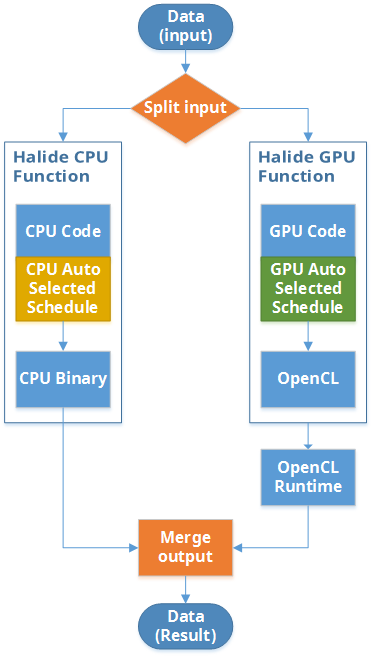
\includegraphics[width=10cm]{img/Framework-SystemFlow.png}
\caption{System Flow}
\label{fig:my_label}
\end{figure}

\begin{figure}[!hbtp]
\centering
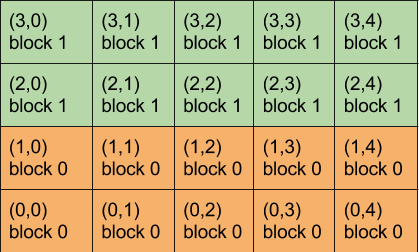
\includegraphics[width=10cm]{img/show_blocks.png}
\caption{Output nubmering.Each elements of output array is shown as a tuple(x,y) with x and y being row and column idex,The number shown in boldface is the block id}
\label{fig:my_label}
\end{figure}

\section{Buffer setup}
\quad \ \ In default way, the Halide will allocate a whole new space in main memory for storage output. If execution device is CPU, output will directly write into the main memory space. However, if the execution device is GPU, Halide will first copy the input main memory to GPU memory. After finishing the computing, Halide will copy the output from GPU memory to main memory. And we have to copy the output from GPU into a new memory space to fit the buffer format of Halide which is shown as Figure ~\ref{fig:Halide_default}. That is, if we use Halide default way to manage memory we have to do memory copy three times (From main memory to GPU, From GPU memory to main memory and from main memory to other main memory spcae to merge output) shown as Figure ~\ref{fig:Halide_default1}.To solve this problem, we have to take over the memory management from Halide by allocating a full size memory and setting the stride for it. In detail, when we  allocate a Halide buffer, it will automatically call a function by Halide to setup the dimensions, boundary and stide for each dimension and create a array as a buffer to save to data. When using our framework we will allocation new buffers for each device, calculate the corresponding boundary and stride for new buffers and set the memory address of the array of the new output buffer to the address of the array of original output buffer which is passed by programmer(Figure ~\ref{fig:memory_new}). By this way, after GPU finish its work, the result can directly copy to the main memory at correctly position.




\begin{figure}[!hbtp]
\centering
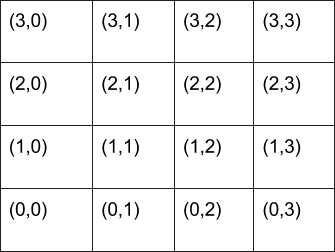
\includegraphics[width=10cm]{img/memory_full.png}
\caption{Original Halide output format}
\label{fig:Halide_default}
\end{figure}

\begin{figure}[!hbtp]
\centering
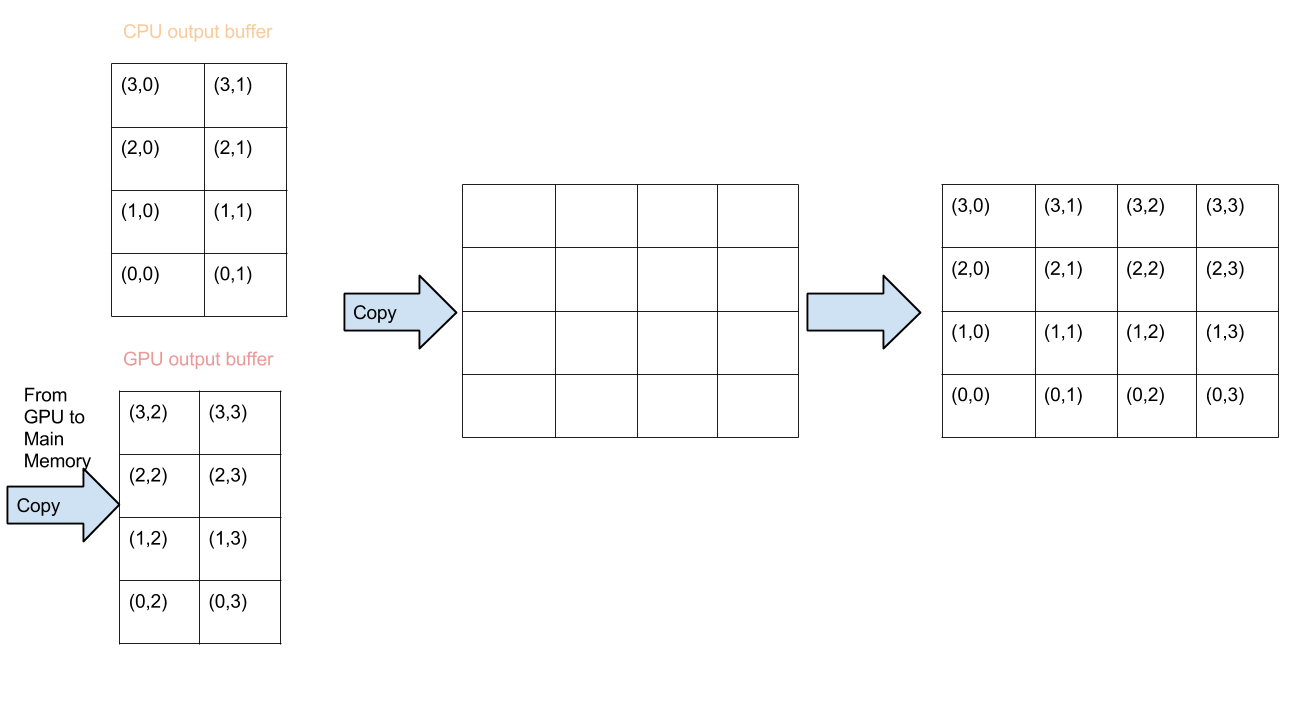
\includegraphics[width=10cm]{img/Memory_copy.png}
\caption{Original Halide output merging}
\label{fig:Halide_default1}
\end{figure}

\begin{figure}[!hbtp]
\centering
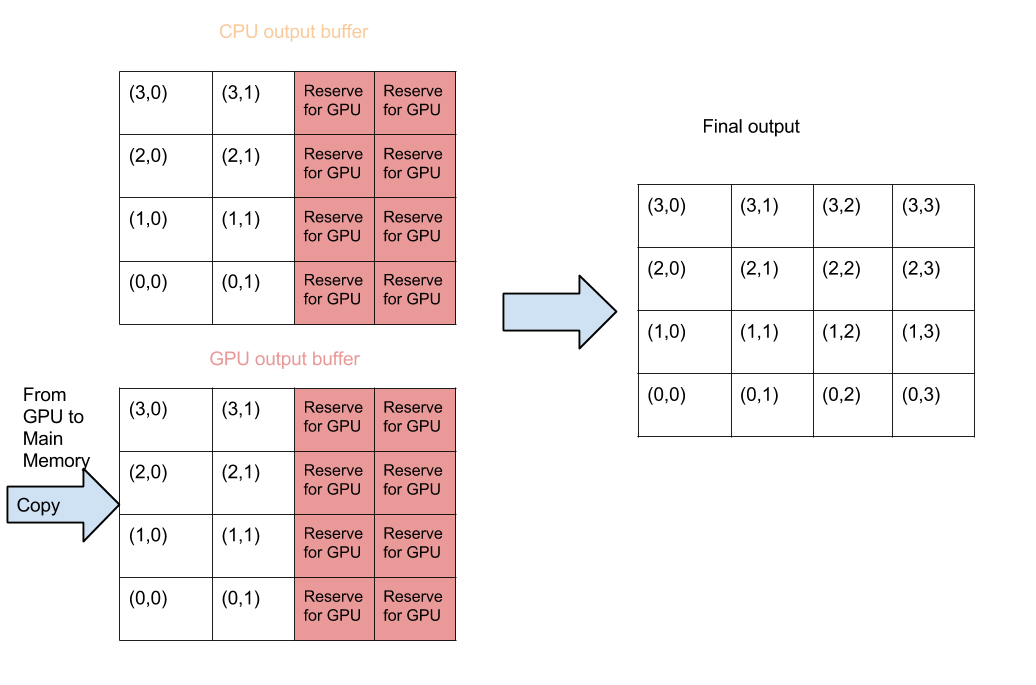
\includegraphics[width=10cm]{img/Memory_copy_new.png}
\caption{Buffer with reserving space}
\label{fig:memory_new}
\end{figure}



\section{Static Dispatch}
\quad\ \ After solving the redundant memory copy problem, we were trying to implement a simple method to achieve the goal that synergistically computing .When the framework is used with specifically workload, we will prepare the output space and set the output stride and other argument by referencing the workload for each CPU and GPU Halide function.  After setting the output for each Halide function, we call Halide function with full size input and the output pointer we prepared for each devices with two thread, one for CPU function and one for GPU. When GPU finished jobs, the output is still kept in GPU memory, the framework should call the function which is provided by Halide to copy the result from GPU memory to main memory. After both CPU and GPU work threads are completed, we will return the final result to the caller. With this implementation, we got about 50\% speedup, the detail experiment result will be shown in next Chapter.

% Furthermore, we implement work stealing skill to speedup static way. By this implementation, we split the workload of CPU into N blocks from 0 to N-1 and the workload of GPU still keep as one block. The CPU thread process blocks sequentially. After GPU finished its workload, The GPU thread will check the status of blocks from N-1 to 0 which should belong to CPU, if there is a block have not been done, GPU will help to process the block. The workload stealing can improve 8\% more compared to static way.

\begin{figure}[hbtp]
\centering
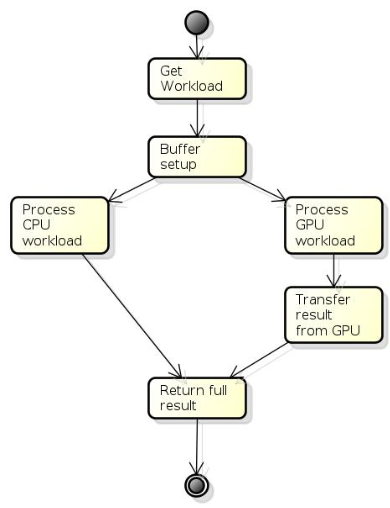
\includegraphics[height=10cm]{img/StaticDispatch.png}
\caption{Flowchart of Static Dispatch}
\label{fig:my_label}
\end{figure}

\section{Dynamic Dispatch}

\quad \ \ By the implementation above, we create an environment to split computation into CPU part and GPU part. However, the decision of the workload on different devices is still  a problem to programmer ,in addition, to get better workload still need an offline profiler to profile the computation. To solve this problem, we implemented a runtime system to manage the workload by split the output into N blocks from 0 to N-1.we let CPU process blocks in increasing order and GPU process blocks from the other end. By this order, CPU and GPU will execute without overlapping.

	To achieve this implementation, we maintain a status table to record the status of each block. When CPU start to process a block, the runtime of CPU part will check the block status is empty or not .If it is empty, it change the status of the block from empty to computing, otherwise, it will stop the computation of CPU part. And CPU runtime will set the parameter and call halide CPU function. After Halide CPU function finished a block, Halide function will directly write the result into output buffer we prepared and the CPU runtime will change the status of the block to finished and process next block. When GPU runtime is going to process a block, it will also check the status of the block like CPU runtime, only when the status of the block is empty, GPU would process the block. When working thread is going to process to the block which is processed by and other devices, the work thread will be terminated by checking the status of next block, that is, if the status of next target block is not empty which means the other part of work is done by another device, the work thread will be terminated. After both work thread finished its jobs, we will return the final result to the caller.
\begin{figure}[hbtp]
\centering
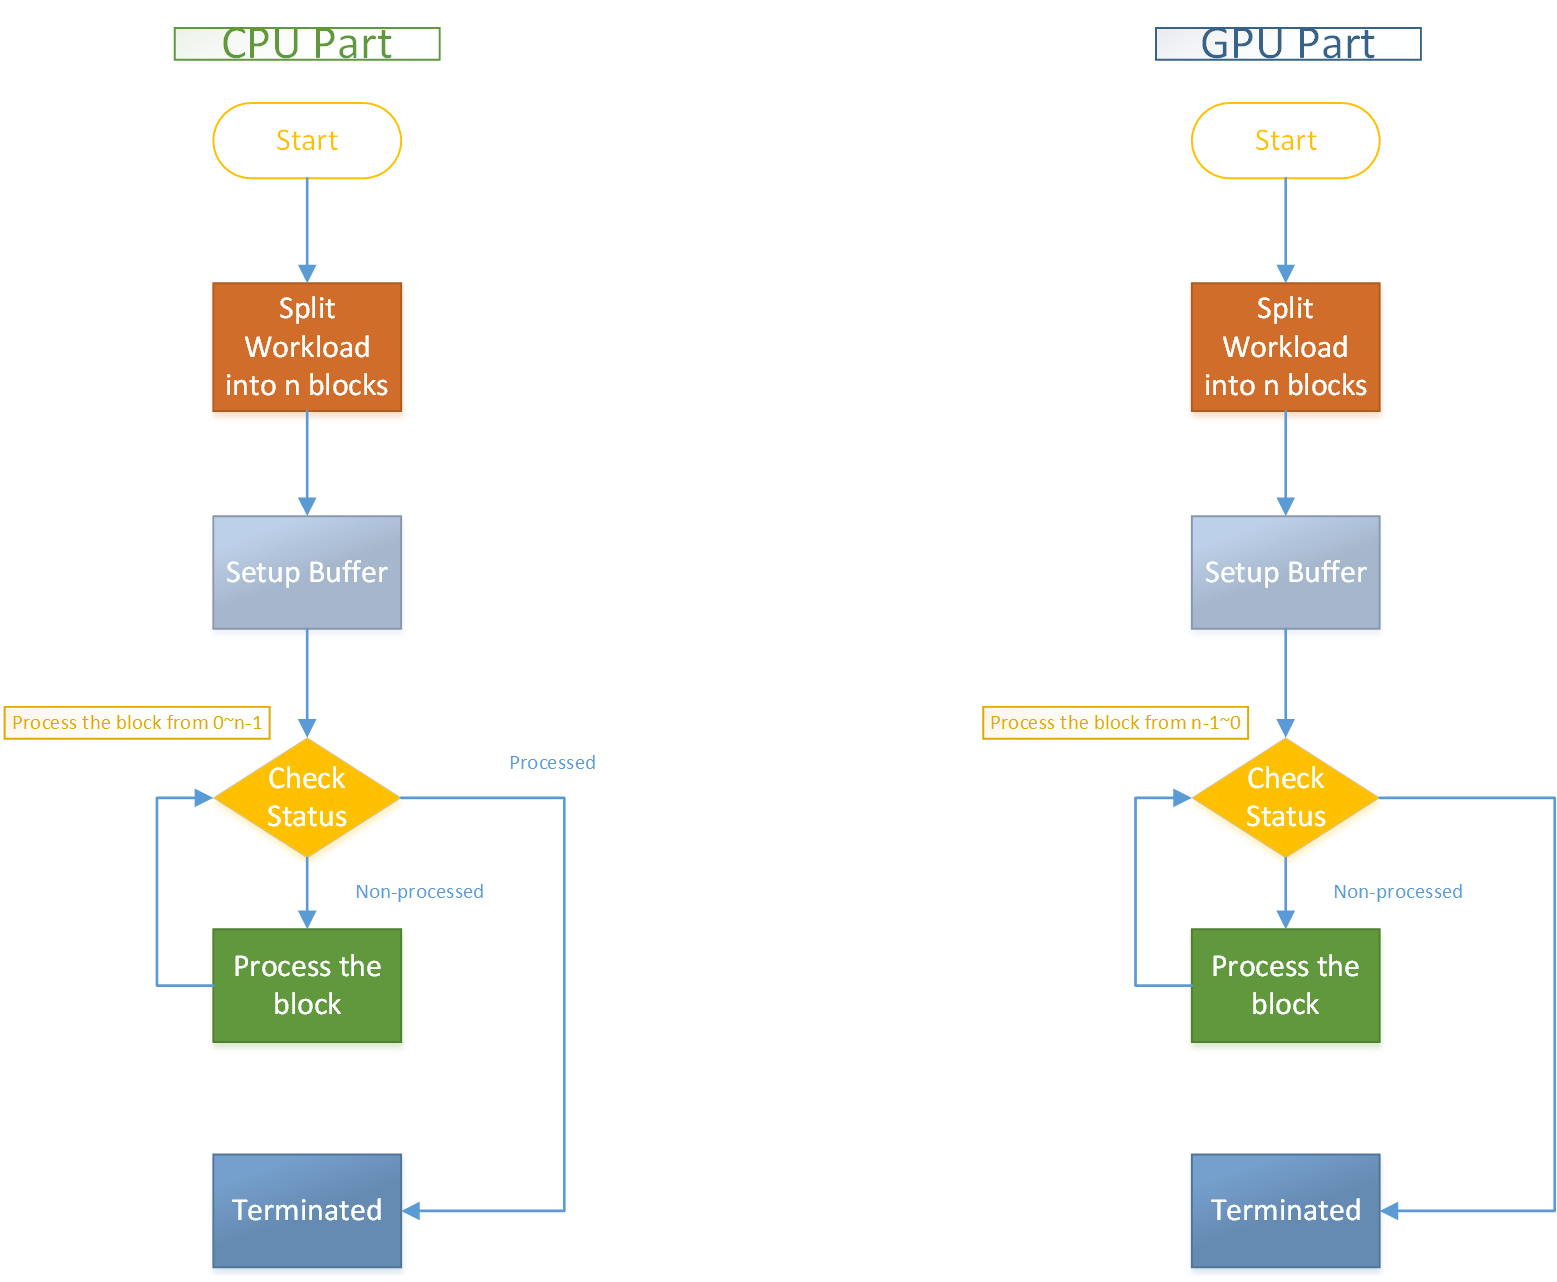
\includegraphics[height=10cm]{img/DynamicDispatchFlow.png}
\caption{Flowchart of Dynamic Dispatch}
\label{fig:my_label}
\end{figure}

\section{Usage of our framework}
\quad \ \ In native Halide, we will get extern functions for different processor which is generated by Halide AOT compiler and will call the function with parameters for the algorithm, input buffer and output buffer in another c++ source file.Here is an example below.
\lstset{language=C++} % Set your language (you can change the language for each code-block optionally)
\begin{lstlisting}[frame=single] % Start your code-block 
//Halide Function
local_laplacian_gpu(levels,alpha/(levels-1),beta,
	input,output); //Halide GPU Function
local_laplacian_cpu(levels,alpha/(levels-1),beta,
	input,output); //Halide CPU Function
\end{lstlisting}

To our framework, you just need to declare a object named StaticDispatch or DynamicDispatch and pass input and output buffer to its constructor.When you want to compute the result just call the function named realize with Halide CPU function, Halide GPU function, workload(if you are using static dispatch), parameters for the algorithm.There are example for using static dispatch and dynamic dispatch below.
\lstset{language=C++} % Set your language (you can change the language for each code-block optionally)
\begin{lstlisting}[frame=single] % Start your code-block 
//Static Dispatch
StaticDispatch static(input,output);
static.realize(local_laplacian_cpu,local_laplacian_gpu,
	workload,levels,alpha/(levels-1),beta);
\end{lstlisting}
\lstset{language=C++} % Set your language (you can change the language for each code-block optionally)
\begin{lstlisting}[frame=single] % Start your code-block 
//Dynamic Dispatch
DynamicDispatch dynamic(input,output);
dynamic.realize(local_laplacian_cpu,local_laplacian_gpu,
	levels,alpha/(levels-1),beta);
\end{lstlisting}

\chapter{Experiments}
\quad \  \ We test the framework with two different application – Bilateral\cite{bilateral} and Local Laplacian\cite{locallaplacian} which are Halide example with tuned schedule for CPU and GPU at three different platform including android platform (Nexus 7) ,detail platform information is shown as table ~\ref{platform1}~\ref{platform2} ,we got at most 57\% improvement with static dispatch and dynamic dispatch compared to best single device. 

\begin{table}[]
\centering
\caption{Test Platform Hardware information}
\label{platform1}
\begin{tabular}{|l|l|l|}
\hline
Platform & CPU & GPU \\ \hline
Android Nexus 7 & \begin{tabular}[c]{@{}l@{}}Quad-core\\ 1.5 GHz Krait\end{tabular} & \begin{tabular}[c]{@{}l@{}}Adreno\\ 320\end{tabular} \\ \hline
PC 1 & \begin{tabular}[c]{@{}l@{}}Intel(R) Core(TM)\\  i5-4590 CPU @ 3.30GHz\end{tabular} & \begin{tabular}[c]{@{}l@{}}ATI Radeon\\ R7 260X\end{tabular} \\ \hline
PC 2 & \begin{tabular}[c]{@{}l@{}}Intel(R) Core(TM)\\  i5-3470 CPU @ 3.20GHz\end{tabular} & \begin{tabular}[c]{@{}l@{}}NVIDIA\\ GTX 750\end{tabular} \\ \hline
\end{tabular}
\end{table}

\begin{table}[]
\centering
\caption{Test Platform software information}
\label{platform2}
\begin{tabular}{|l|l|l|}
\hline
Platform & Compiler & OpenCL Runtime \\ \hline
Android Nexus 7 & \begin{tabular}[c]{@{}l@{}}Android Ndk r10c\\ Halide release\_2015\_06\_03\end{tabular} & Adreno driver for nexus 7 \\ \hline
PC 1 & \begin{tabular}[c]{@{}l@{}}Clang++ 3.6\\ Halide release\_2015\_06\_03\end{tabular} & AMD APP SDK 3.0 Beta \\ \hline
PC 2 & \begin{tabular}[c]{@{}l@{}}Clang++ 3.6\\ Halide release\_2015\_06\_03\end{tabular} & Nvidia driver 337 \\ \hline
\end{tabular}
\end{table}



At the beginning, we have to prove that it is possible we can improve performance by split work into two partitions. So we took Bilateral and Local Laplacian as our benchmark, in each case we gave same input and try to make halide to compute partial output from 10\% to 90\% on CPU and GPU to show the relationship between execution time and workload. 
\begin{figure}[hbtp]
\centering
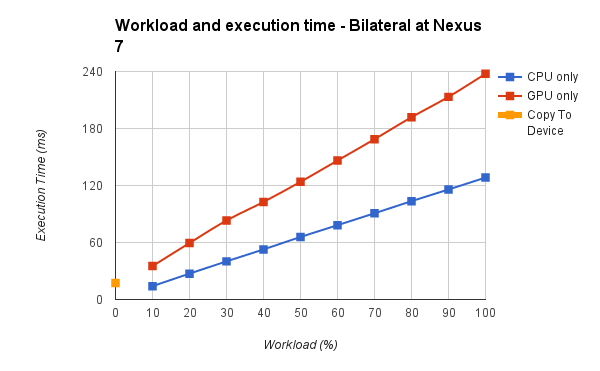
\includegraphics[width=12cm]{img/Result-WorkloadbetweenCPUandGPU(Bilateral@Nexus7).png}
\caption{Result-Bilateral at Nexus 7 }
\label{fig:my_label}
\end{figure}

\begin{figure}[hbtp]
\centering
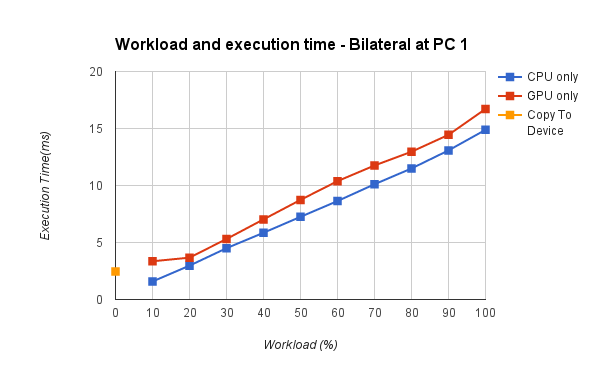
\includegraphics[width=12cm]{img/Result-WorkloadbetweenCPUandGPU(Bilateral@PC1).png}
\caption{Result-Bilateral at PC 1 }
\label{fig:my_label}
\end{figure}

\begin{figure}[hbtp]
\centering
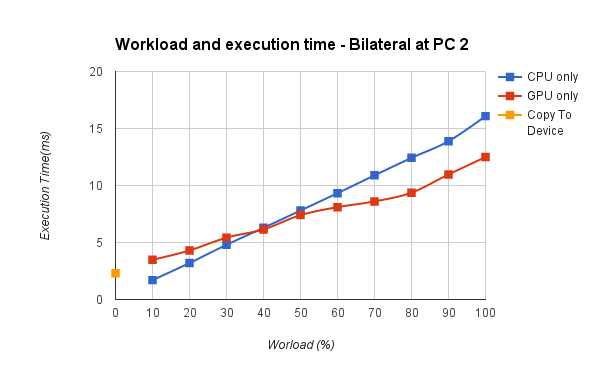
\includegraphics[width=12cm]{img/Result-WorkloadbetweenCPUandGPU(Bilateral@PC2).png}
\caption{Result-Bilateral at PC 2 }
\label{fig:my_label}
\end{figure}

According to experiment result we got, we notice that we could improve performance by split workload into two different devices when processing Bilateral filter. 

%We also test another filter local laplacian the relation between workload and execution time. 
\begin{figure}[hbtp]
\centering
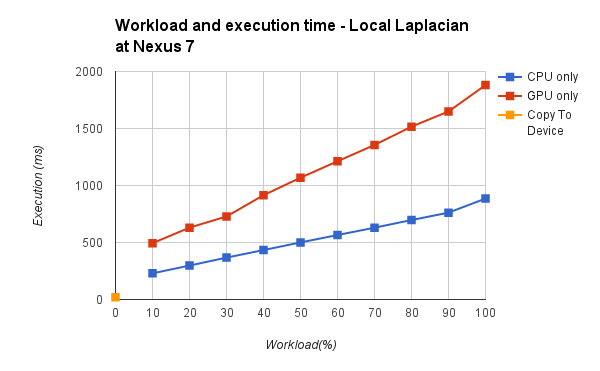
\includegraphics[width=12cm]{img/Result-WorkloadbetweenCPUandGPU(LocalLaplacian@Nexus7).png}
\caption{Result-Loca lLaplacian at Nexus 7 }
\label{fig:my_label}
\end{figure}

\begin{figure}[hbtp]
\centering
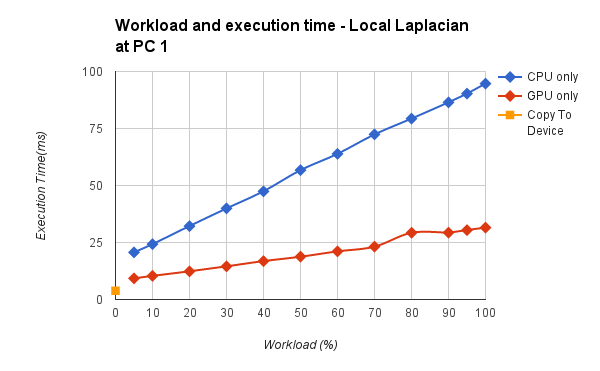
\includegraphics[width=12cm]{img/Result-WorkloadbetweenCPUandGPU(LocalLaplacian@PC1).png}
\caption{Result-Local Laplacian at PC 1 }
\label{fig:my_label}
\end{figure}

\begin{figure}[hbtp]
\centering
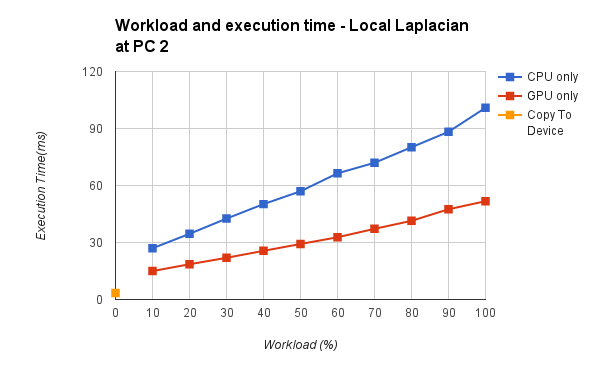
\includegraphics[width=12cm]{img/Result-WorkloadbetweenCPUandGPU(LocalLaplacian@PC2).png}
\caption{Result-Local Laplacian at PC 2 }
\label{fig:my_label}
\end{figure}

We notice that the trend line of Local laplacian is similar to Bilateral. However, there is one little part which is different to Bilateral, that is, according to the trend line, when the workload of bilateral filter equals to zero, the execution time of CPU also equals to zero and the execution time of GPU would equal to the time of copying to device, but the trend line of Local laplacian is not, the trend line of CPU will be higher than zero when the workload equals to zero  and the trend line of GPU will also be higher than the time of coping to device, which means if we split work of local laplacian into 2 or more partition the execution of two or more partition will greater than only 1 partition and it will increase when we split work into more partition, which also implies that we may not get same improvement between static dispatch and dynamic dispatch when the framework handling the case like local laplacian.

\section{Static Dispatch}

\quad \ \ To test static dispatch we assign different workload to CPU and GPU to test the best performance on Static Dispatch. Totally, there are 9 composition between CPU and GPU workload.

In those results, the high peak of the CPU workload and the mapping GPU workload (GPU workload reverse in the diagram) should be the ideal execution time of static dispatch and the line is the real execution time of static dispatch. We got about 1.21x , 1.55x and 1.16x at Nexus7, PC 1 and PC2 respectively when processing bilateral filter compared to best single device. We also got 1.24x, 1.03x and 1.11 speedup improvement at Nexus7, PC 1 and PC2 respectively  when processing Local Laplacian filter compared to best single device. 

However, in the diagrams of Bilateral filter, the static dispatch (the line) is higher than the peak. The gap between high peak and the real static execution time should be overhead of OpenCL runtime, we will profile and discuss the runtime information on next section.

\begin{figure}[hbtp]
\centering
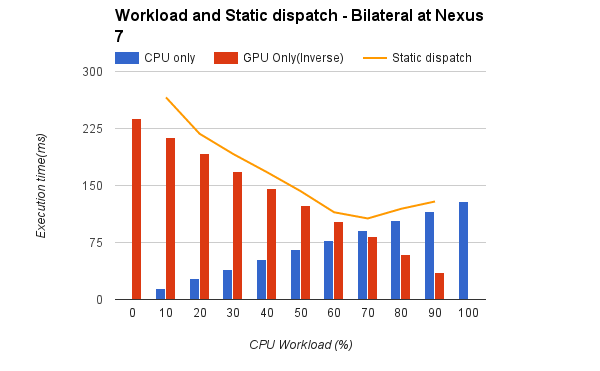
\includegraphics[width=12cm]{img/Result-WorkloadAndStaticDispatch(Bilateral@Nexus7)}
\caption{Result- Bilateral at Nexus 7 }
\label{fig:my_label}
\end{figure}

\begin{figure}[hbtp]
\centering
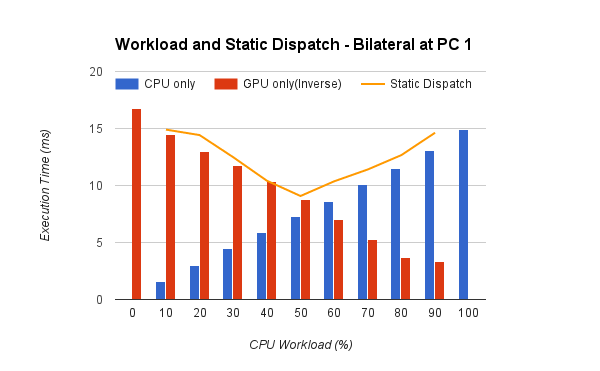
\includegraphics[width=12cm]{img/Result-WorkloadAndStaticDispatch(Bilateral@PC1)}
\caption{Result- Bilateral at PC 1 }
\label{fig:my_label}
\end{figure}

\begin{figure}
\centering
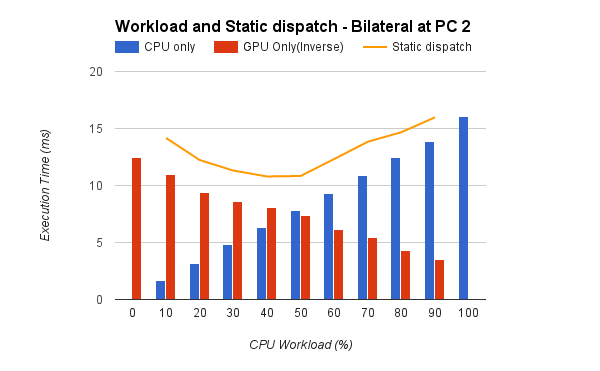
\includegraphics[width=12cm]{img/Result-WorkloadAndStaticDispatch(Bilateral@PC2)}
\caption{Result- Bilateral at PC 2 }
\label{fig:my_label}
\end{figure}


\begin{figure}[hbtp]
\centering
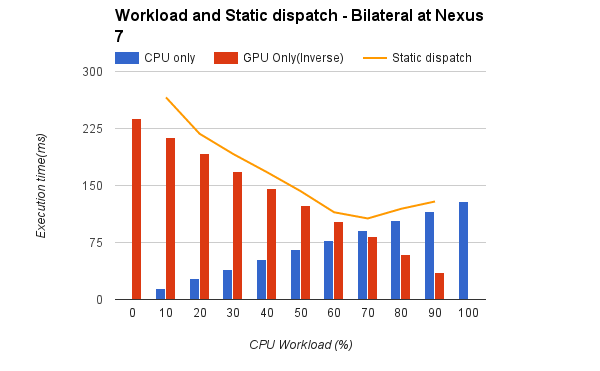
\includegraphics[width=12cm]{img/Result-WorkloadAndStaticDispatch(Bilateral@Nexus7)}
\caption{Result- Local Laplacian at Nexus 7 }
\label{fig:my_label}
\end{figure}

\begin{figure}[hbtp]
\centering
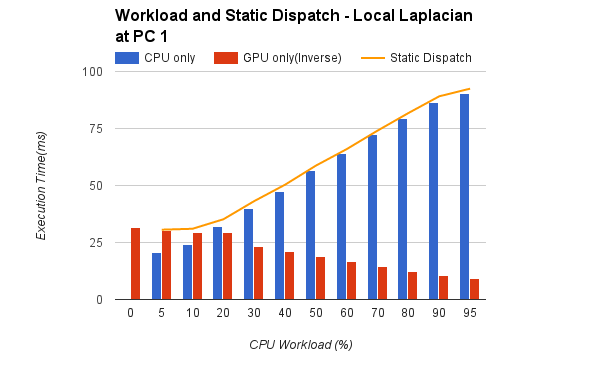
\includegraphics[width=12cm]{img/Result-WorkloadAndStaticDispatch(LocalLaplacian@PC1)}
\caption{Result- Local Laplacian at PC 1}
\label{fig:my_label}
\end{figure}

\begin{figure}[hbtp]
\centering
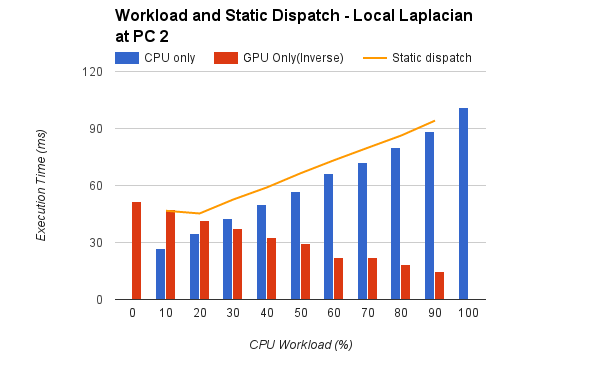
\includegraphics[width=12cm]{img/Result-WorkloadAndStaticDispatch(LocalLaplacian@PC2)}
\caption{Result- Local Laplacian at PC2 }
\label{fig:my_label}
\end{figure}

\section{Dynamic Dispatch}
\quad \  \ After implement static dispatch, we want to implement an easier way to programmer to use both devices, we also implement dynamic dispatch and hope it could be effective as static dispatch.

\begin{figure}[!hbtp]
\centering
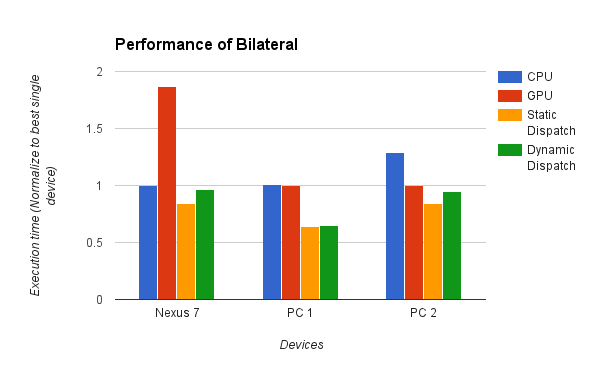
\includegraphics[width=12cm]{img/PerformanceOfBilateral.png}
\caption{Performance of Bilateral filter. For each devices, execution time is shown normalized to the best performing single device – CPU-only or GPU-only.}
\label{fig:my_label}
\end{figure}

\begin{figure}[!hbtp]
\centering
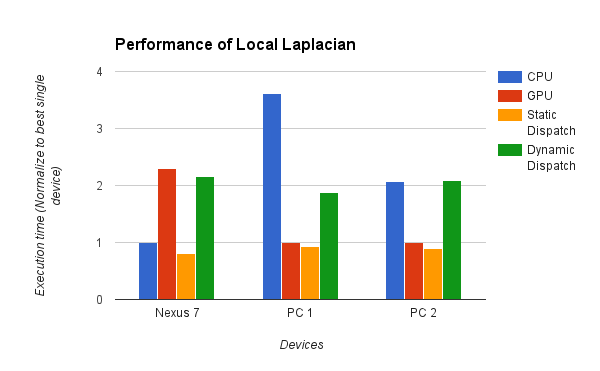
\includegraphics[width=12cm]{img/PerformanceOfLocalLaplacian.png}
\caption{Performance of Local Laplacian  filter. For each devices, execution time is shown normalized to the best performing single device – CPU-only or GPU-only.}
\label{fig:my_label}
\end{figure}

According to the results, it shows that dynamic dispatch will be slower than static dispatch especially when processing filter like local laplacian which matchs our assumption before. It is because filter like local laplacian which will refer to all input data cannot split into multiple blocks or it will refer to all input redundantly. 

\section{Profile OpenCL Runtime information}

\quad \  \ The gap between ideal static execution real static execution should be the overhead of OpenCL runtime information.To prove that, we profile OpenCL runtime information to figure out the bottleneck of our framework. We profile the runtime information of GPU only with processing specific percentage workload and static dispatch with same workload to compare the execution of each stage of OpenCL API.


\begin{figure}[!hbtp]
\centering
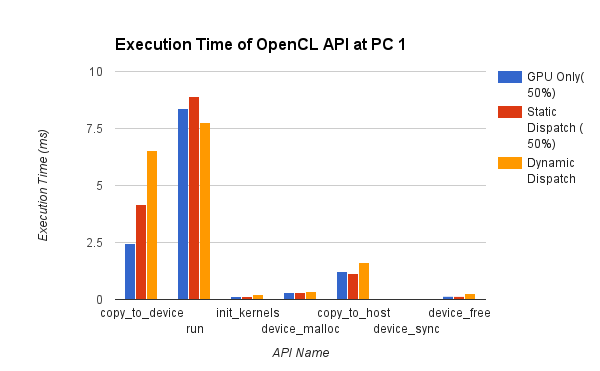
\includegraphics[width=12cm]{img/ExecutionTimeOfAPI(Bilateal@PC1).png}
\caption{Execution time Of OpenCL API at PC1 each API is normalized to GPU only.}
\label{fig:my_label}
\end{figure}

\begin{figure}[!hbtp]
\centering
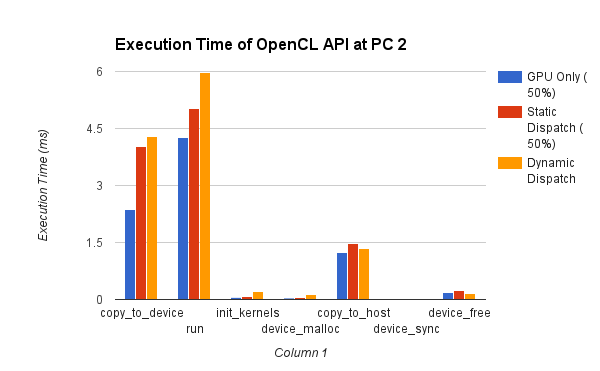
\includegraphics[width=12cm]{img/ExecutionTimeOfAPI(Bilateal@PC2).png}
\caption{Execution time Of OpenCL API at PC2 each API is normalized to GPU only.}
\label{fig:my_label}
\end{figure}

\section{CUDA and OpenCL}
\quad \  \ In addition to OpenCL, Halide also support CUDA as the language of GPU which means our framework should also support CUDA, so we also measured the performance and make a comparison between CUDA and OpenCL when processing bilateral and local laplacian at PC2.



\begin{figure}[hbtp]
\centering
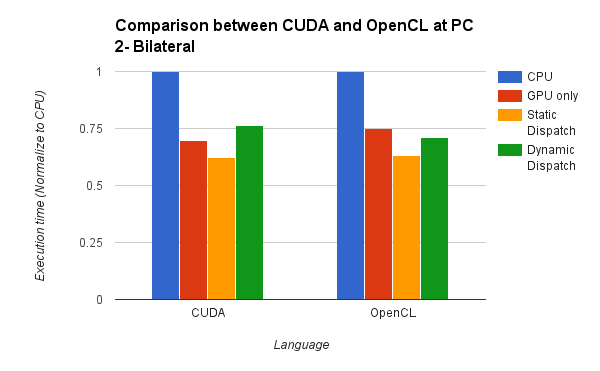
\includegraphics[width=12cm]{img/ComparisonBetweenCUDAAndOpenCL(Bilateral).png}
\caption{Comparison between CUDA and OpenCL when processing Bilateral Filter. Each time is normalized to CPU execution time}
\label{fig:my_label}
\end{figure}

\begin{figure}[hbtp]
\centering
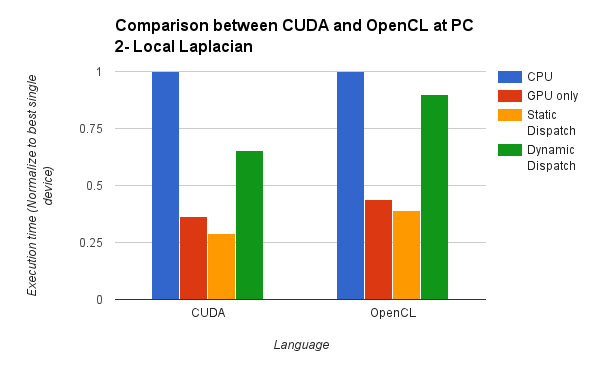
\includegraphics[width=12cm]{img/ComparisonBetweenCUDAAndOpenCL(LocalLaplacian).png}
\caption{Comparison between CUDA and OpenCL when processing Local Laplacian Filter. Each time is normalized to CPU execution time}
\label{fig:my_label}
\end{figure}

\section{Different Input Size}
\quad \  \ To test the influence of different input size, we also experiment different input with 8192*6960 pixel.According to our results, PC 1 can similar to our predict execution time, however, PC 2 still slower to our predict execution time even if we enlarge input size .To figure out the reason, we also profile the API time of this input size, in next section, we will discuss the results.

\begin{figure}[!hbtp]
\centering
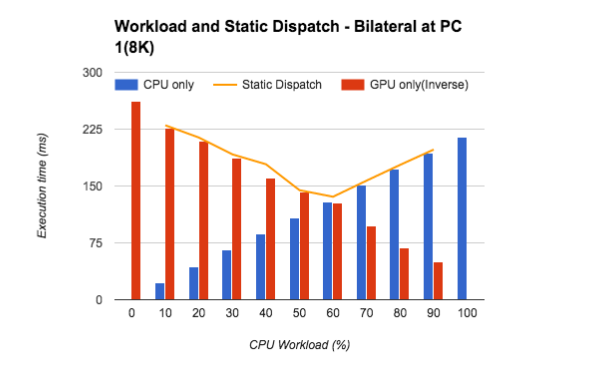
\includegraphics[width=12cm]{img/WorkloadAndStaiticDispatch-BilateralAtPC1(8K).png}
\caption{Result- Bilateral at PC 1 with 8K input size}
\label{fig:my_label}
\end{figure}

\begin{figure}[!hbtp]
\centering
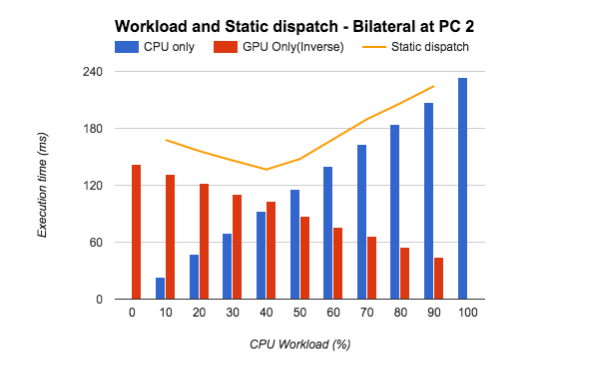
\includegraphics[width=12cm]{img/WorkloadAndStaiticDispatch-BilateralAtPC2(8K).png}
\caption{Result- Bilateral at PC 2 with 8K input size}
\label{fig:my_label}
\end{figure}


\section{OpenCL API exection time with larger size}
\quad \  \ After profiling OpenCL API execution time, Figure ~\ref{fig:ExeTime8KPC2} shows that the gap between GPU only and static dispatch still exists in PC 2 when input size became to 8192*6960.

\begin{figure}[!hbtp]
\centering
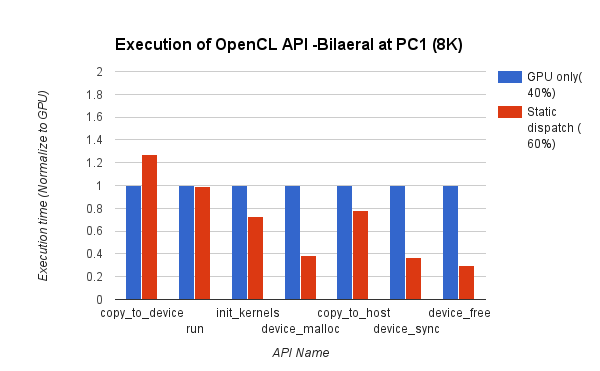
\includegraphics[width=12cm]{img/ExecutionofOpenCLAPI-BilateralatPC1(8K).png}
\caption{Execution time of openCL API - Bilateral at PC 1 (8K)}
\label{fig:ExeTime8KPC1}
\end{figure}

\begin{figure}[!hbtp]
\centering
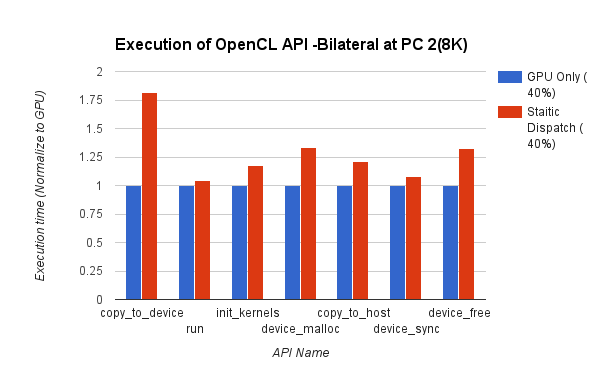
\includegraphics[width=12cm]{img/ExecutionofOpenCLAPI-BilateralatPC2(8K).png}
\caption{Execution time of openCL API - Bilateral at PC 2 (8K)}
\label{fig:ExeTime8KPC2}
\end{figure}




\chapter{Conclusion}
Our work is to make framework which is easy to use and can get improvement by using synergistic computation. In this paper, we use Halide as our language and make a runtime on Halide to build a synergistic and easy computing environment. 
According to our experiment, we could improve the execution time by splitting the workload into 2 or more partitions and dispatching them to CPU and GPU.  Also, our framework could get at most 1.55x speedup when processing case like Bilateral compared to fastest single device, but when processing algorithm like local laplacian we can get only few improvement when using static dispatch and may not get improvement when using dynamic dispatch because of the feature of the algorithm. However, even if we can get at most 1.55x speedup improvement, we still cannot get ideal performance improvement which we predict. But when kernel computing takes more percentage in the whole execution, in other word, when the algorithm become more complex, we could reduce the influence of OpenCL runtime and get more improvement.
In short, with the feature of Halide, we build a synergistic computing environment that is easy to program, tune performance and take advantage of both CPU and GPU to computing the jobs.



%\appendix

\backmatter

\addcontentsline{toc}{chapter}{\bibname}
\bibliographystyle{unsrt}

% Your bibliography goes here
\nocite{*}
\bibliography{thesis}

\end{document}

